\begin{figure}[t]
    \centering
    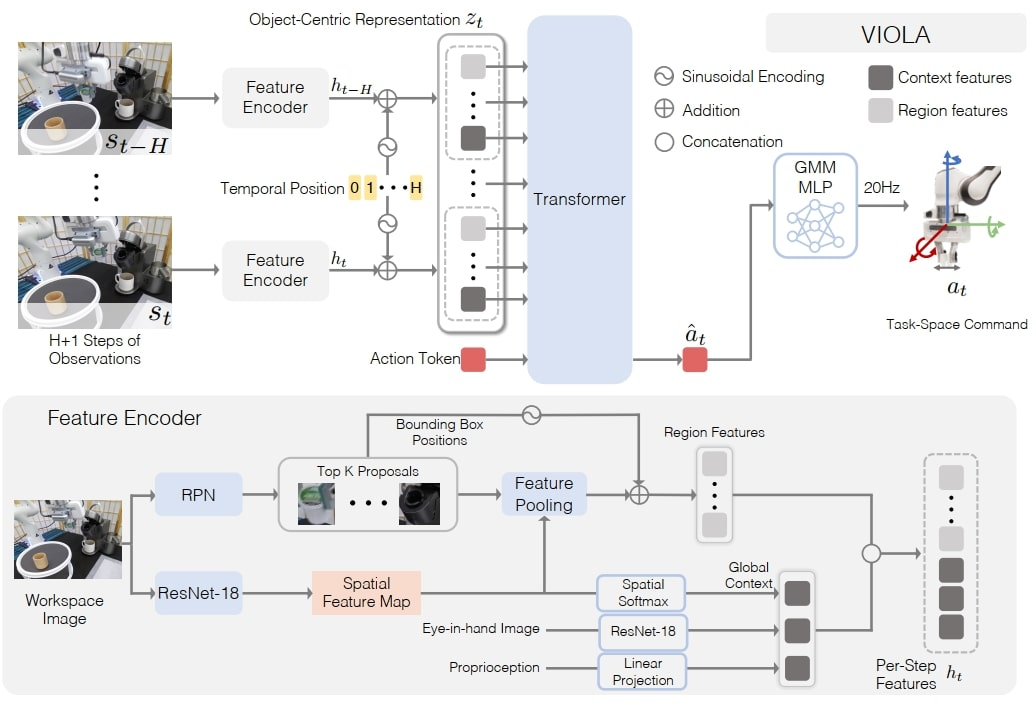
\includegraphics[width=0.7\textwidth]{figures/images/viola/viola_architecture.jpg}
        \caption{The VIOLA architecture proposed in \cite{zhu2023viola}. (Top) The overall control architecture is based on a Transformer module that processes a stack of \textit{per-step features} $h_{t}$, obtained from the Feature Encoder, to generate a final action embedding, which is then input into a GMM policy. (Bottom) The Feature Encoder builds both local and global features. Local features correspond to regions of interest extracted by the RPN. Global features are obtained by processing the workspace image, the image from the camera on the gripper, and proprioceptive information.
        }
    \label{fig:viola_architecture}
    
\end{figure}

\begin{figure}[t]
    \centering
    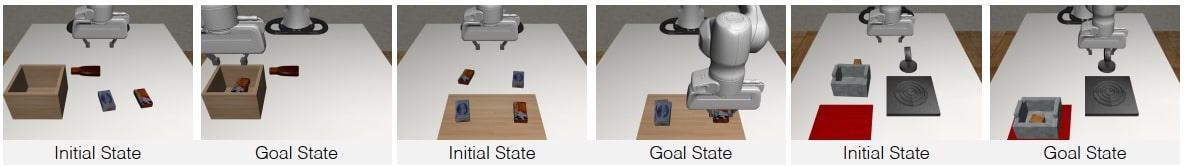
\includegraphics[width=0.9\textwidth]{figures/images/viola/viola_task.jpg}
    \caption{Simulation tasks on which the VIOLA \cite{zhu2023viola} method was tested. (Left) Sorting task. (Center) Stacking task. (Right) BUDS-Kitchen task}
    \label{fig:viola_task}
    
\end{figure}
